\documentclass[10pt]{article}
\usepackage[a4paper,margin=1.6cm]{geometry}
\usepackage{graphicx,booktabs,amsmath,amssymb,enumitem,xcolor,float}
\usepackage[hidelinks]{hyperref}
\setlist{nosep,leftmargin=1.3em}
\setlength{\parindent}{0pt}\setlength{\parskip}{4pt}
\newcommand{\ok}{\textcolor{green!50!black}{\checkmark}}
\newcommand{\no}{\textcolor{red!70!black}{$\times$}}
\title{\vspace{-1.2cm}Position histories vs integrator: 1D underdamped cos well}
\date{26 November 2026}
\begin{document}
\maketitle\vspace{-0.6cm}

\begin{itemize}
\item \textbf{Fit:} NPNEq on one MD trajectory, 2M frames, $\gamma=1$, $kT=1$, $dt=0.005$, A: $x\le-0.35$, B: $x\ge0.35$.
\item \textbf{Fit settings:} warm-up 1000 iterations at envelope 1, then 10000 at envelope 0.01, $\gamma_\mathrm{fit}=0.1$, ny 6.
\item \textbf{Inputs:} \textbf{x, v} (recorded velocity, no history); \textbf{x + history [0, 1]} or \textbf{[0, 1, 2, 4]}
  ($x$ only, basis in $(x(t-d), x(t))$, shift \texttt{'r(t)'}).
\item \textbf{Integrators:} EM (Euler--Maruyama), BBK (toytis), ASE (Vanden-Eijnden--Ciccotti).
\item \textbf{Exact committor:} grid solve for each integrator's own step.
\item \textbf{Which seed:} the one with the lowest RMS. Full tables: \texttt{README.md}.
\end{itemize}

\section*{Result}
\begin{center}
\begin{tabular}{llll}
\toprule
integrator & x, v & x + history [0, 1] & x + history [0, 1, 2, 4] \\
\midrule
EM  & \ok\ (RMS 0.012) & \textbf{\ok\ (0.012)} & \ok\ (0.015) \\
BBK & \ok\ (0.007) & \textbf{\no\ (0.030)}: $Z_q$ +20\,\% at short lags & partial (0.020): $Z_q$ +4\,\% \\
ASE & \ok\ (0.018) & \textbf{\no\ (0.033)}: $Z_q$ +20\,\% at short lags & partial (0.027): $Z_q$ +4\,\% \\
\bottomrule
\end{tabular}\\[2pt]
{\small RMS is per frame, against the exact committor.}
\end{center}

\begin{itemize}
% \item \textbf{ASE offset (about $-0.01$ to $-0.02$ in every ASE fit):} sampling noise of the single run used
%   (run 0 of 50, about 5500 transitions), not a bias of the method or the reference.
%   \begin{itemize}
%   \item In run 0, the MD outcome committor over free frames is 0.490, against 0.498 for the exact one.
%   \item Over runs 0--9, the MD outcome and the exact committor agree per $(x, v)$ bin: mean $-0.0004$, RMS 0.005.
%   \end{itemize}
\item x, v works for every integrator, provided the seed is good. Poor seeds stall at RMS 0.036--0.046 for all three.
\item History [0, 1] matches x, v for EM only. For BBK and ASE it fails, with the same $Z_q$ signature in both.
\item History [0, 1, 2, 4] reduces the failure but does not remove it. BBK and ASE again give the same $Z_q$ pattern
  (EM and BBK at seed 1, one seed each; the ASE notebook seeds 1--3 give 0.025--0.027).
\item Cross-entropy and AUC do not detect the failure. $Z_q$, or the comparison with the exact committor, does.
\end{itemize}

\begin{figure}[H]\centering
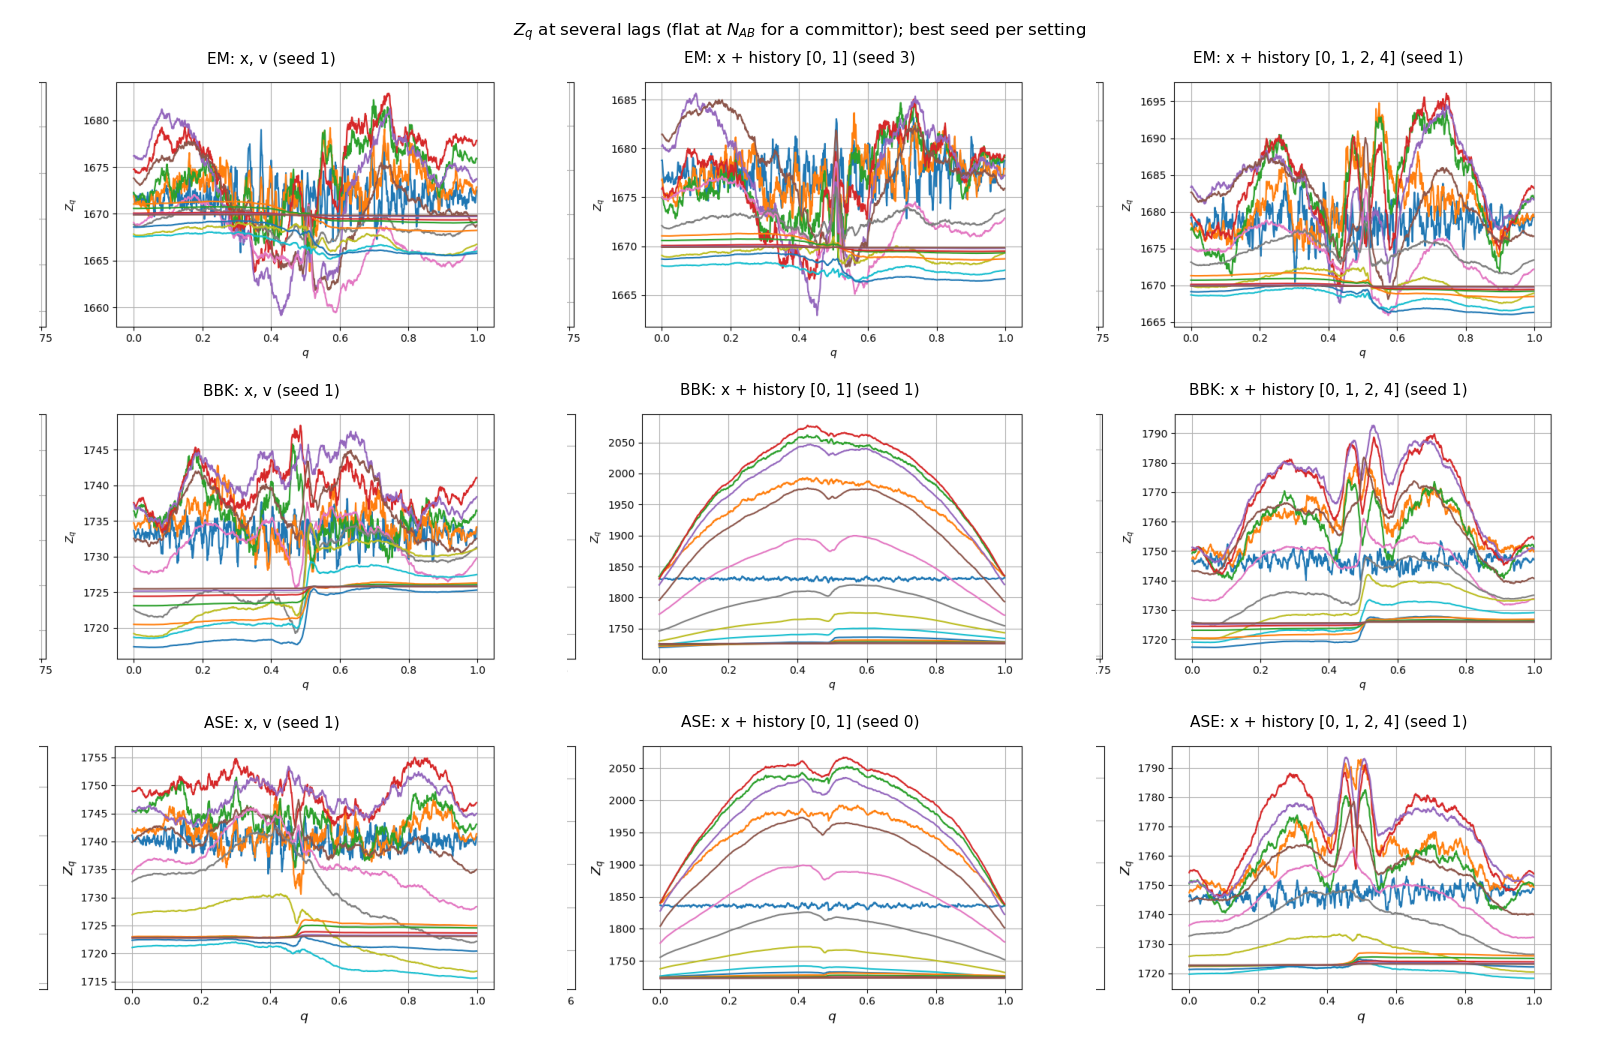
\includegraphics[width=\textwidth]{simple_zq.png}
\caption{$Z_q$ at several lags (flat at $N_{AB}$ for a committor), best seed per setting.}
\end{figure}

\section*{Best seed per setting}
Each row: $F(q)$, $F(q)$ in the natural coordinate, $Z_q$ \;|\; $q(x,v)$ \;|\; fit $-$ exact \;|\; exact.

\begin{figure}[H]\centering
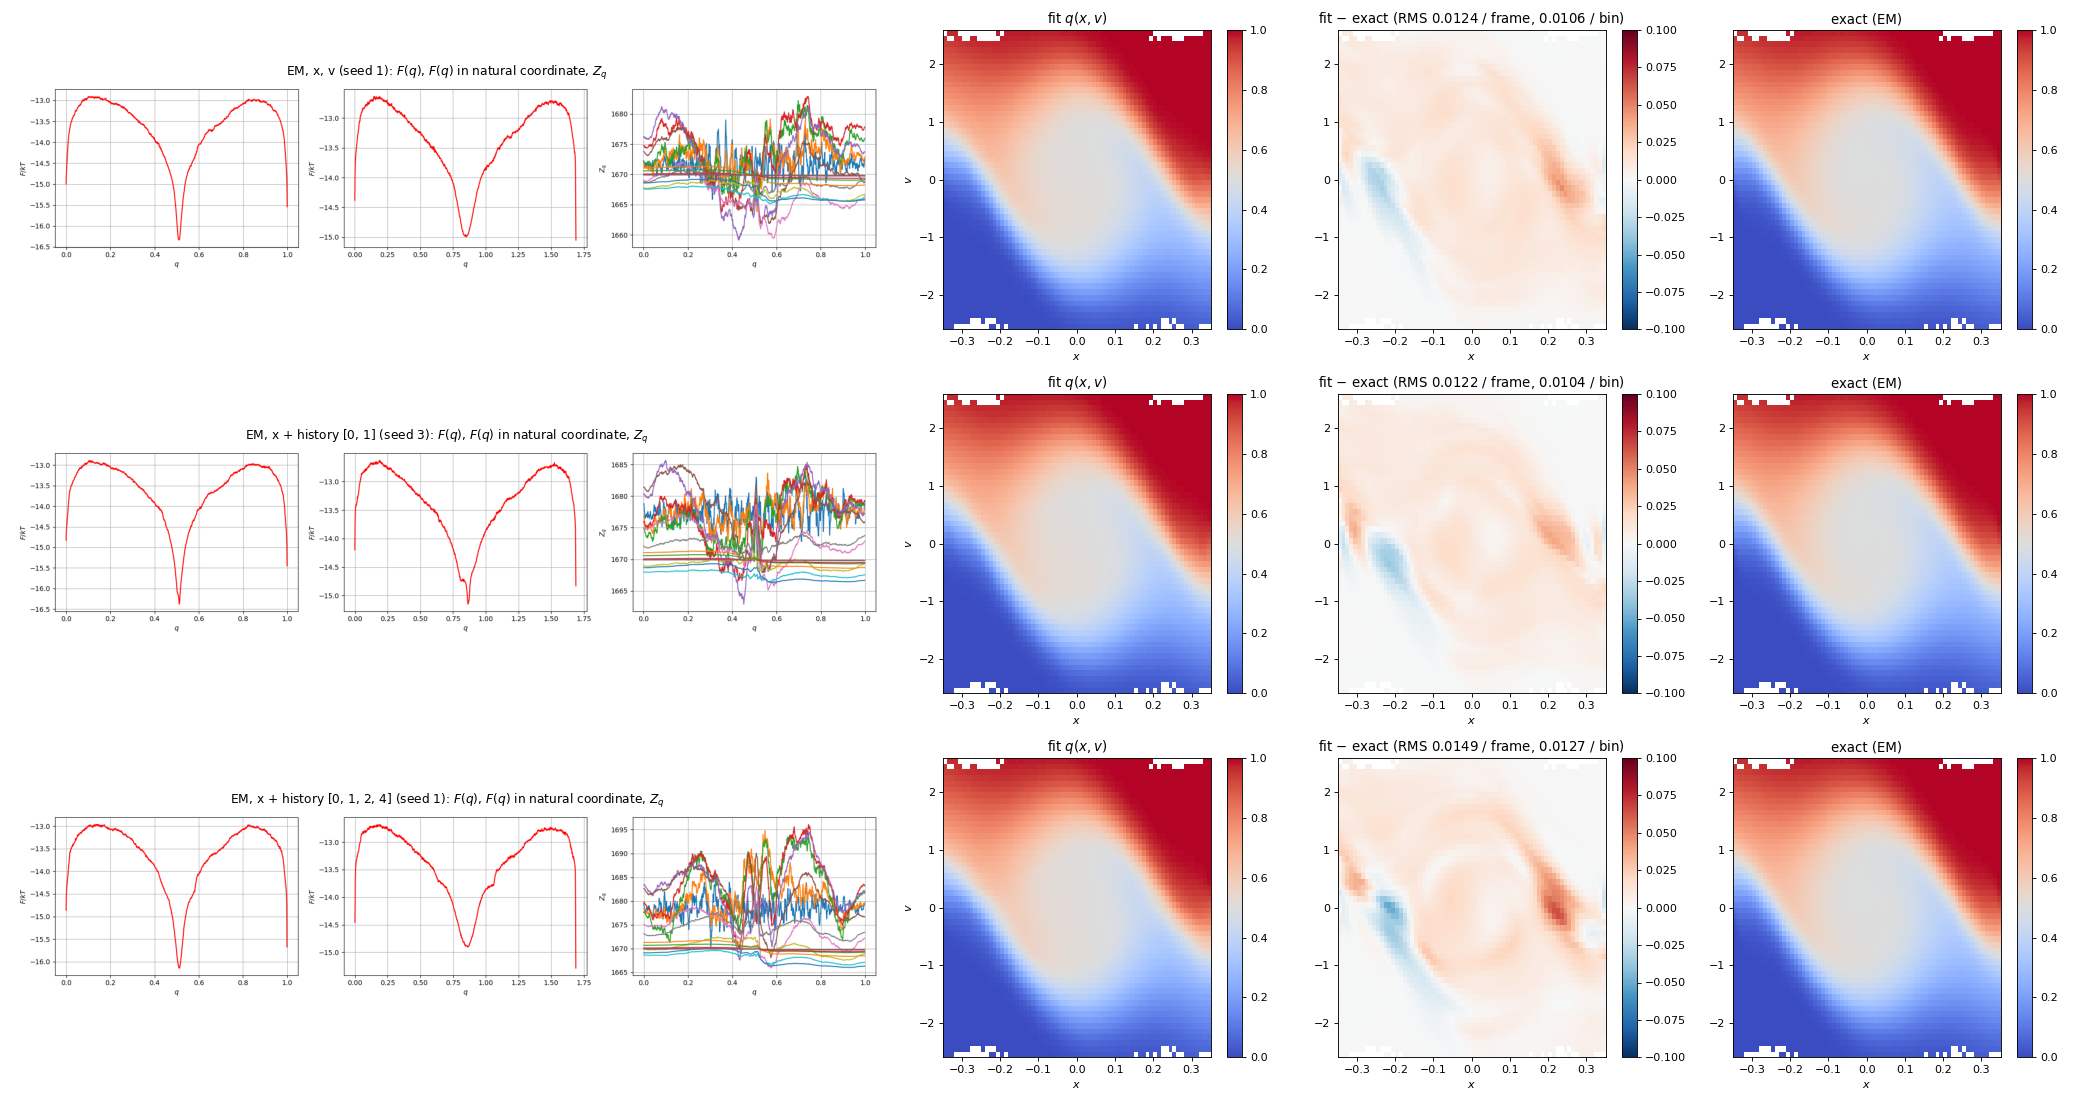
\includegraphics[width=\textwidth]{simple_best_EM.png}\caption{EM.}
\end{figure}
\begin{figure}[H]\centering
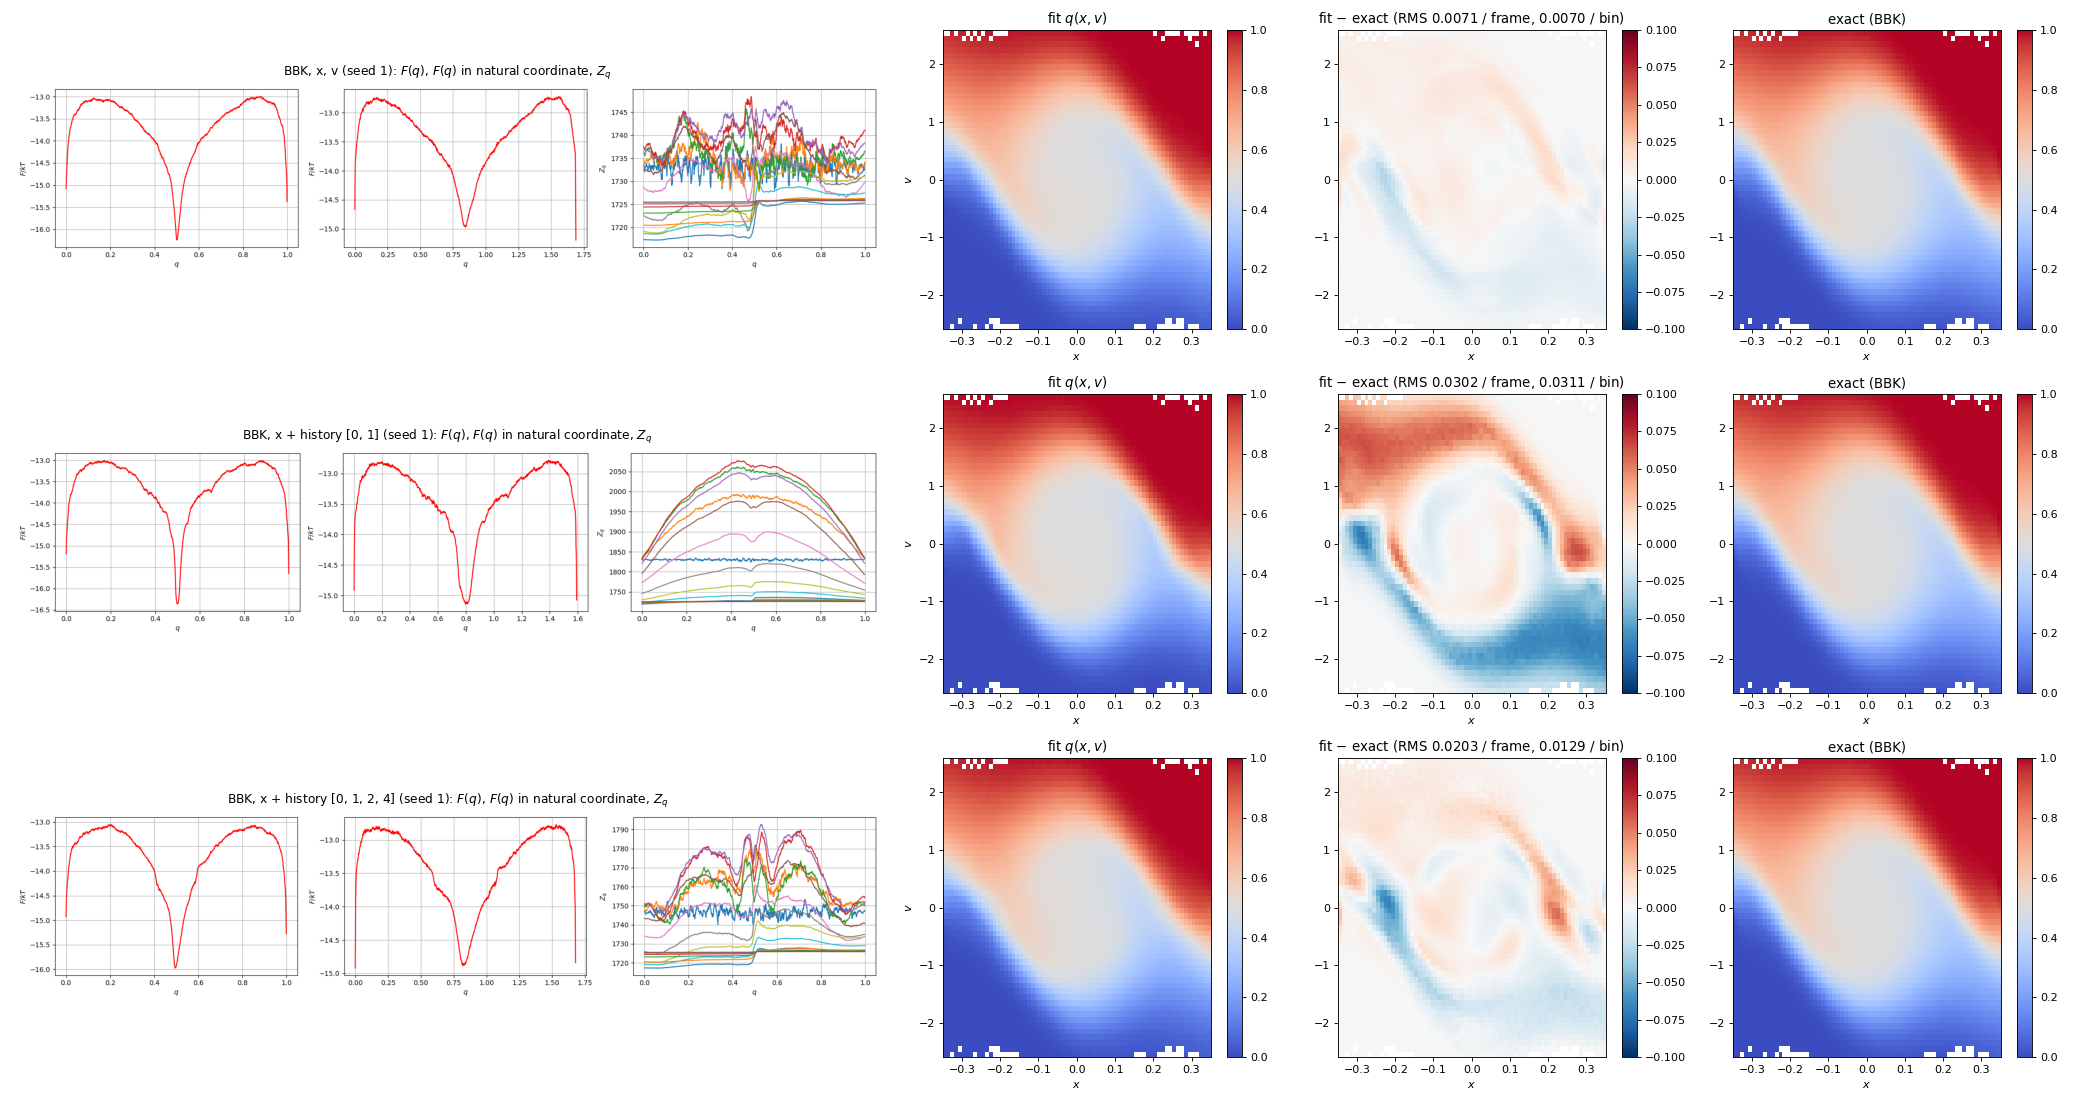
\includegraphics[width=\textwidth]{simple_best_BBK.png}\caption{BBK.}
\end{figure}
\begin{figure}[H]\centering
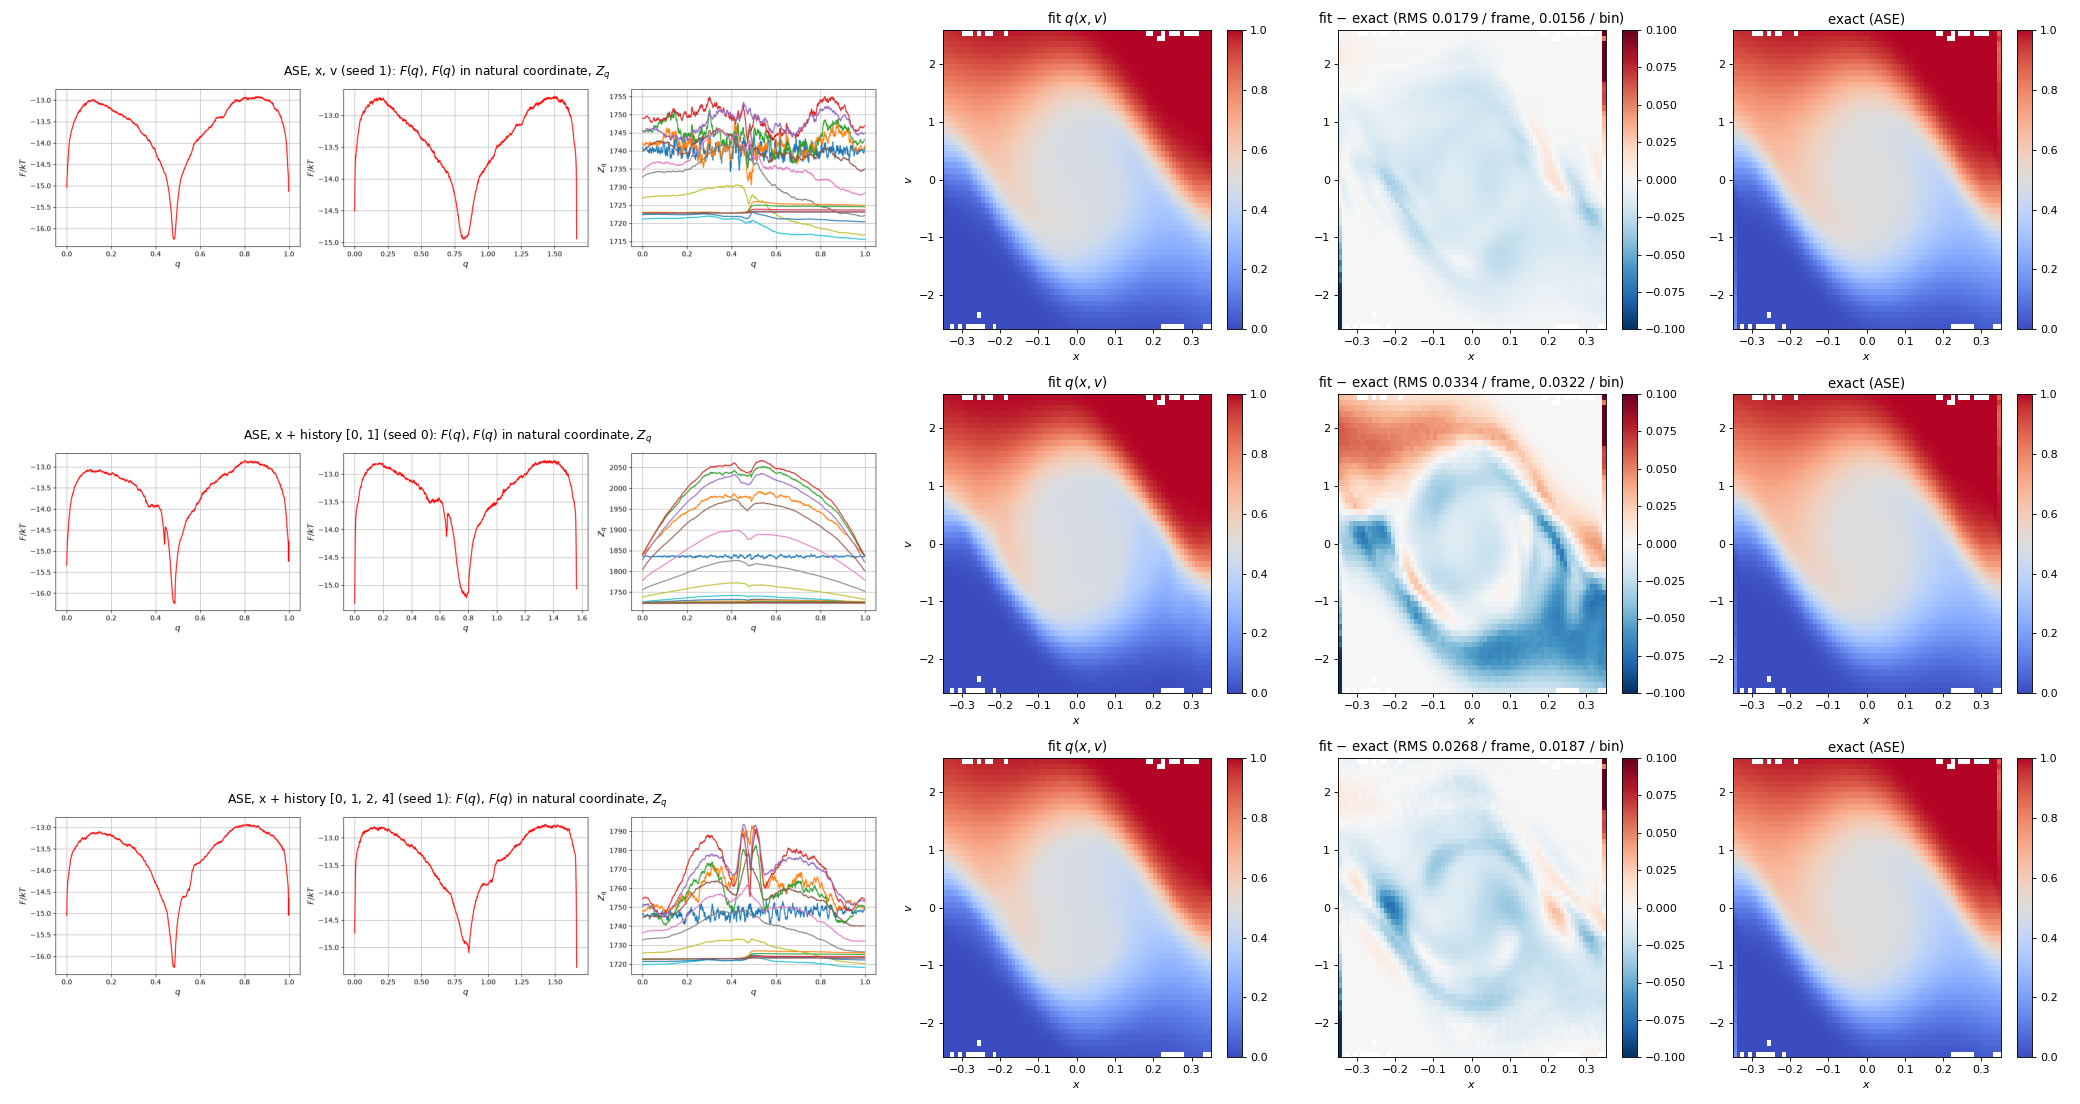
\includegraphics[width=\textwidth]{simple_best_ASE.png}\caption{ASE.}
\end{figure}

\begin{itemize}
\item \textbf{BBK and ASE with history [0, 1]:} a smooth error of about $\pm0.05$, the same for every seed. $q$ is too
  high at large positive $v$, too low at large negative $v$, with rings along the energy contours: the energy
  diffusion is biased. There are no edges, so this is not a convergence problem.
\item \textbf{EM with history [0, 1]:} about $\pm0.02$, as good as x, v.
\item \textbf{[0, 1, 2, 4] for BBK and ASE:} the same shape at about half the size. Per bin, RMS drops from
  0.031--0.032 to 0.013 (BBK) and 0.019 (ASE).
\end{itemize}

\section*{Example of a bad x, v seed (BBK, seed 2)}
\begin{figure}[H]\centering
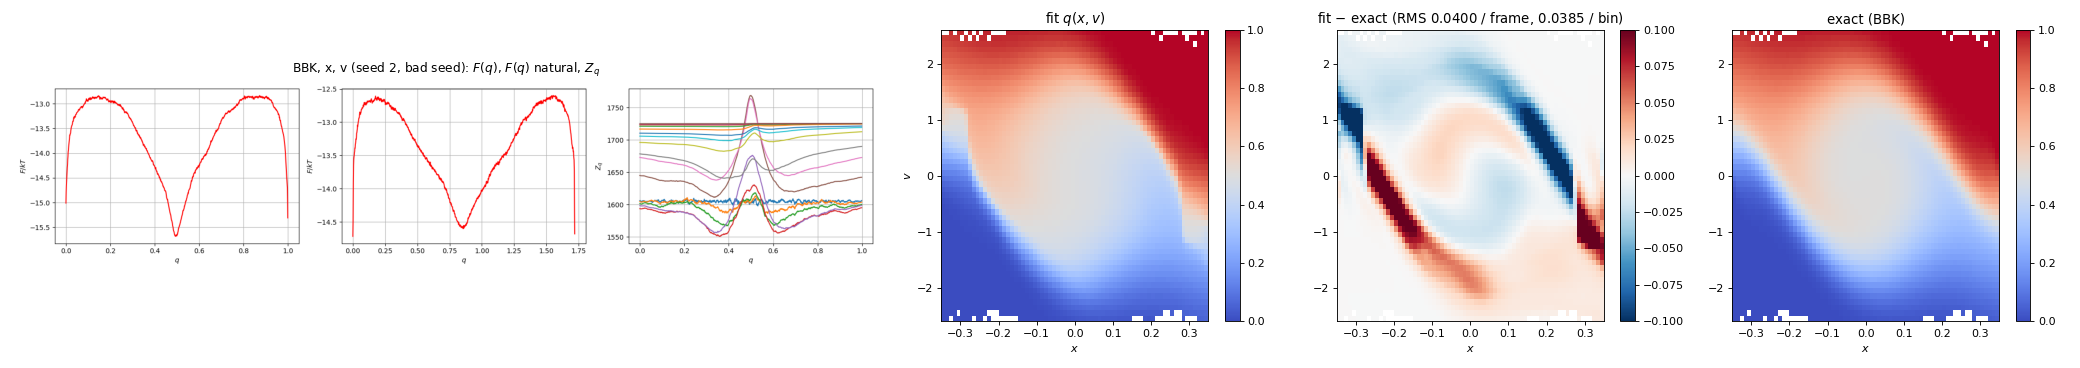
\includegraphics[width=\textwidth]{simple_bad.png}\caption{BBK, x, v, seed 2: $F(q)$, $F(q)$ natural, $Z_q$ \;|\; $q(x,v)$ \;|\; fit $-$ exact \;|\; exact.}
\end{figure}
\begin{itemize}
\item \textbf{Same data and settings as the good seed 1 (RMS 0.007);} only the seed differs. RMS 0.040 per frame,
  max\_sd\_zq 34 against 5.
\item \textbf{Map:} vertical edges at $x\approx\pm0.28$, and narrow diagonal bands along the contours with errors up
  to $\pm0.1$. Elsewhere $q$ is close to the exact one.
\item \textbf{$Z_q$:} about 7\,\% too low at short lags ($\approx$ 1600 against $N_{AB}\approx$ 1725), with a bump at
  $q\approx0.5$. This differs from the history failure, which is 20\,\% too high and smooth.
\item \textbf{Same in all three integrators:} seeds 2 and 3 stall at 0.036--0.046 (EM 0.036 / 0.040, BBK 0.040 / 0.041,
  ASE 0.044 / 0.046), and seed 1 is good in all three.
\item \textbf{Cause:} the lag-1 (x, v) fit depends on its start, i.e. on which CV and envelope
  centre the first iterations draw. 
% \item \textbf{Remedy:} a lag-16 (x, v) fit reached the noise floor on the 6M-frame BBK data (same document).
\end{itemize}

% LARGER FIT LAG SECTION: commented out for now, remove the leading "% " from the lines below to include it
% \section*{Larger fit lag (\texttt{delta\_t = delta\_t\_stride = SUB})}
% \begin{itemize}
% \item \textbf{Setup:} the update uses only every SUB-th frame. The history stays on the fine grid: [0, 1] is
%   $x(t-1)$ (``fine''); ``coarse'' is [0, SUB]. A transition stops at the first frame in A or B, also between the
%   subsampled frames.
% \item \textbf{Prediction:} the hidden velocity noise has a fixed size per step, while the velocity noise over SUB
%   steps grows with SUB. For BBK and ASE the history bias should shrink roughly as 1/SUB.
% \end{itemize}
% \begin{center}\small
% \begin{tabular}{lllrlll}
% \toprule
% integrator & fit & SUB & iter. & RMS / frame & RMS / bin & max\_sd\_zq \\
% \midrule
% EM  & x + hist. [0, 1] (fine), seed 1 & 20 & 16000 & 0.018 & 0.015 & 68 \\
% BBK & x + hist. [0, 1] (fine), seed 1 & 20 & 16000 & \textbf{0.020} & \textbf{0.010} & 76 \\
% ASE & x, v, seed 111 & 2 & 16000 & n/a & n/a & $\approx$ 20 \\
% ASE & x + hist. [0, 1] (fine), seed 111 & 2 & 16000 & n/a & n/a & $\approx$ 41 \\
% ASE & x + hist. [0, 2] (coarse), seed 111 & 2 & 16000 & n/a & n/a & $\approx$ 70 \\
% ASE & x + hist. [0, 1] (fine), seed 111 & 20 & 16000 & n/a & n/a & $\approx$ 64 \\
% ASE & x + hist. [0, 1] (fine), seed 111 & 50 & 16000 & 0.051 (0.043 at 6000) & n/a & $\approx$ 350 \\
% \bottomrule
% \end{tabular}\\[2pt]
% ASE stride runs: from the notebook's plots and printout; their $q$ arrays are not here.
% \end{center}
% \begin{itemize}
% \item \textbf{BBK, lag 20:} the history bias is gone. RMS per bin is 0.010 (lag 1: 0.031), close to BBK x, v
%   (0.007), and the smooth $v$-dependent band in the error map has disappeared.
% \item \textbf{RMS per frame stays at 0.02:} each frame still carries the scatter of the velocity noise it cannot
%   see. The per-bin average removes that scatter.
% \item \textbf{EM, lag 20:} accurate with 20$\times$ fewer transitions (0.018, against 0.012 at lag 1). There is
%   nothing to gain, since EM history already works at lag 1.
% \item \textbf{$Z_q$:} flat at $N_{AB}$ for lags $\ge 20$. The lags below 20 wiggle: EM overshoots, BBK
%   undershoots. That is why max\_sd\_zq (68, 76), which includes the short lags, is not the right measure here.
%   A lag-$\Delta$ fit should be judged at lags $\ge\Delta$.
% \item \textbf{$F(q)$ is wiggly:} $q$ is only constrained over 20-frame steps, so it can vary on shorter scales.
% \item \textbf{ASE, SUB 2:} fine history beats coarse (max\_sd\_zq $\approx$ 41 vs $\approx$ 70).
% \item \textbf{ASE, SUB 50:} gets worse with more iterations, with speckle at high $|v|$. With 27.6k transitions the
%   polynomial basis overfits its sparse corners.
% \end{itemize}
% \begin{figure}[H]\centering
% 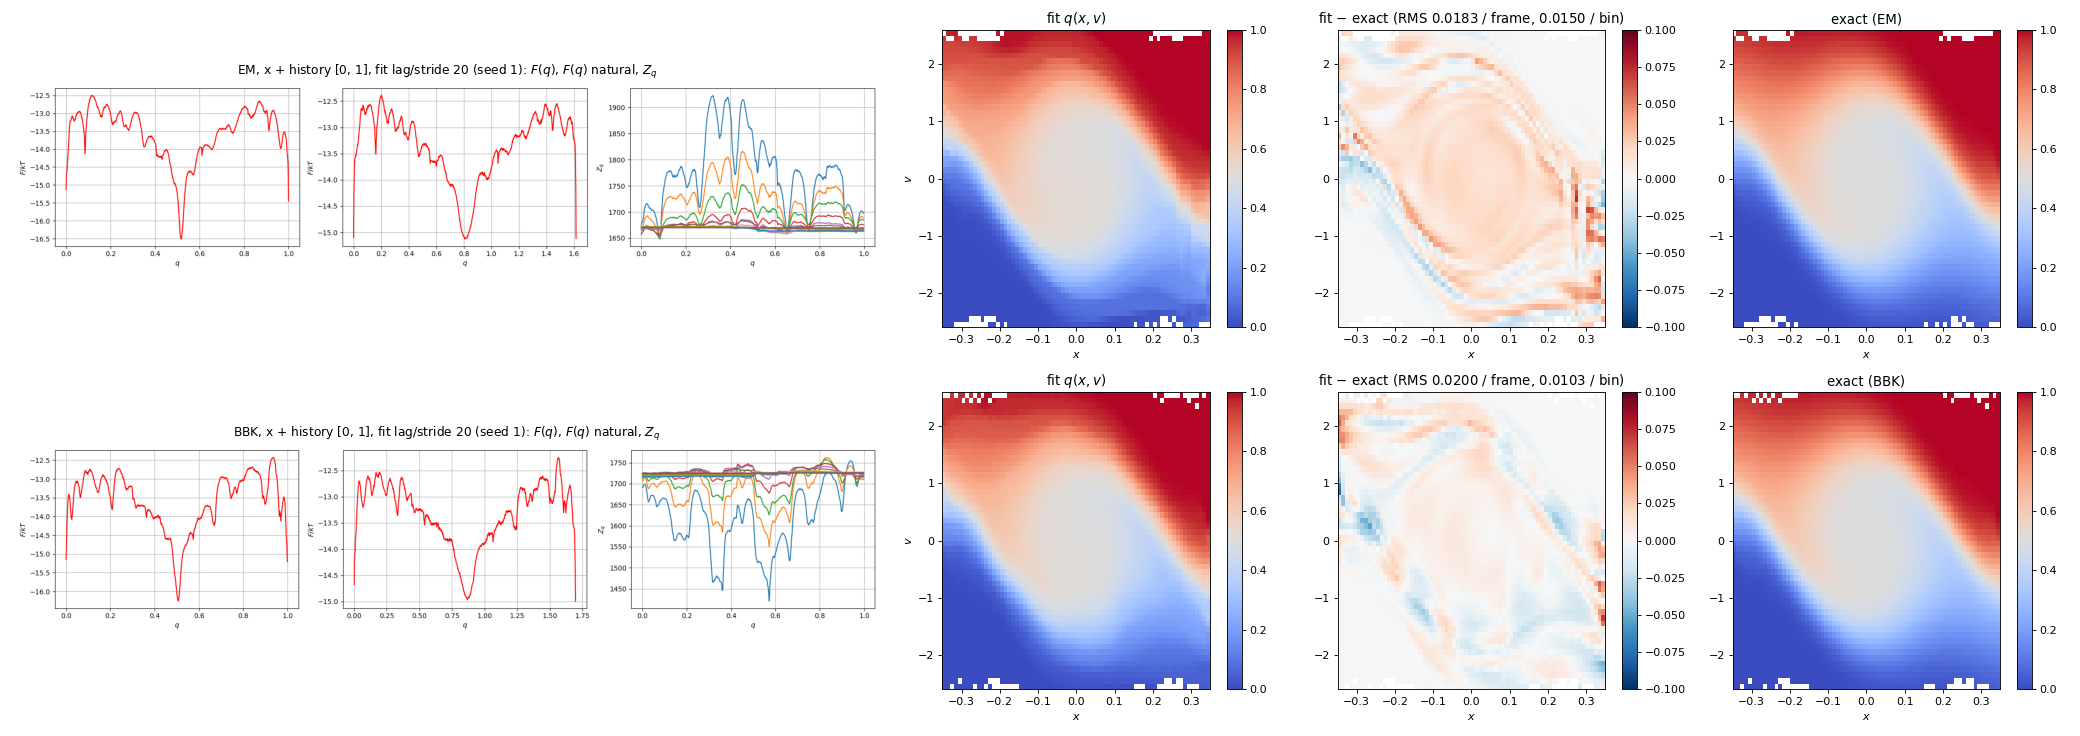
\includegraphics[width=\textwidth]{simple_stride.png}\caption{EM and BBK, x + history [0, 1], fit lag/stride 20.}
% \end{figure}
% \begin{figure}[H]\centering
% 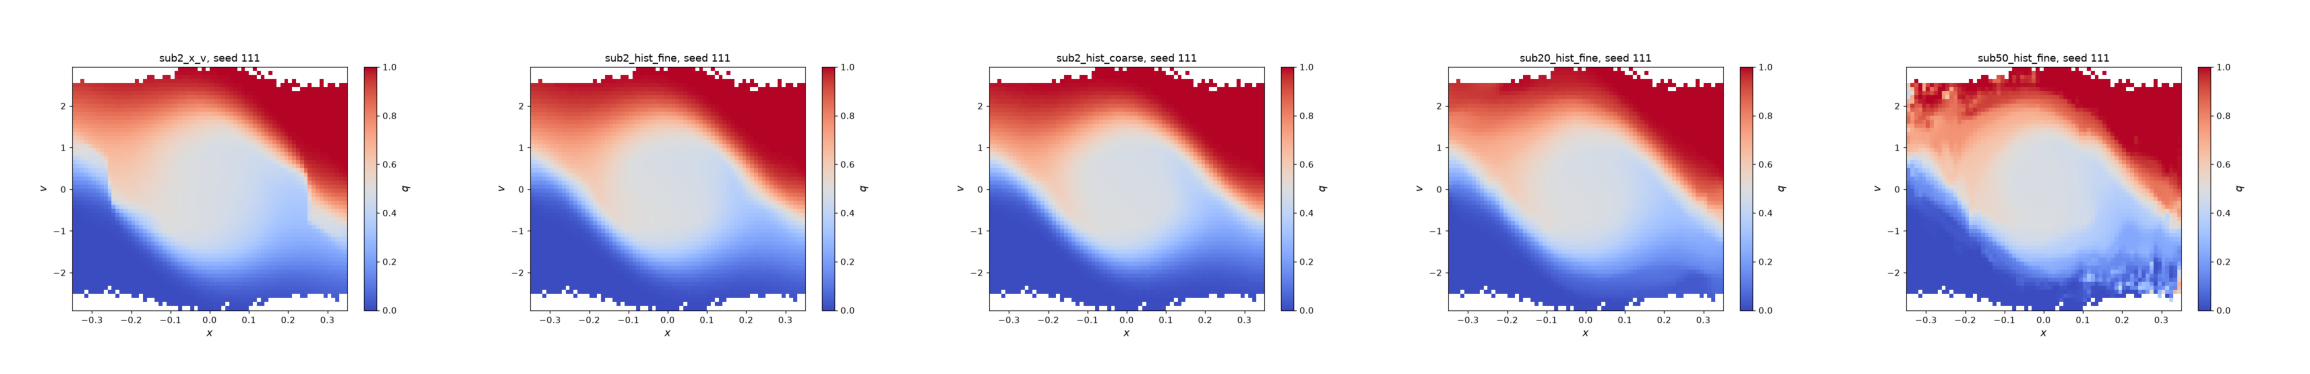
\includegraphics[width=\textwidth]{fig_stride_ase_maps.png}\caption{ASE stride runs: $q(x,v)$ (notebook images).}
% \end{figure}
%
\section*{New history type (EM, BBK, ASE)}
\begin{itemize}
\item \textbf{Setup:} $x$ + history [0, 1], \texttt{history\_type = ['y(t-d),y(t)', 'y(t-d),r(t-d)']}, one drawn at random each
  iteration; the second uses the earlier committor estimate $r(t-d)$ and $x(t-d)$. Seed 2611, 1000 warm-up + 25000 main
  iterations; same data, settings and exact references as above; one seed per integrator.
\end{itemize}
\begin{center}\small
\begin{tabular}{lllll}
\toprule
integrator & old type: RMS / frame & new type: RMS / frame & new type: RMS / bin & $Z_q$ (from plot) \\
\midrule
EM  & 0.012 & 0.0138 & 0.0117 & within $\pm1$\,\% \\
BBK & 0.030 & \textbf{0.0166} & \textbf{0.0073} & within $\pm1$\,\%, dip $-1.6$\,\% at $q\approx0.5$ \\
ASE & 0.033 & \textbf{0.0238} & 0.0166 & within $\pm1$\,\% \\
\bottomrule
\end{tabular}
\end{center}
\begin{itemize}
\item \textbf{BBK and ASE:} the $+20$\,\% $Z_q$ excess and the smooth $v$-dependent error band are gone. What remains is a
  localized error of about $\pm0.05$ in two streaks near $x\approx\pm0.22$, $v\approx0$, in all three integrators (EM included).
\item \textbf{BBK per bin 0.0073} is close to BBK $x, v$ (0.007). \textbf{EM} is unchanged. \textbf{ASE} keeps the uniform
  offset of about $-0.01$ of every ASE fit.
\item \textbf{One seed each:} the figure does not show the seed-to-seed spread.
\end{itemize}
\begin{figure}[H]\centering
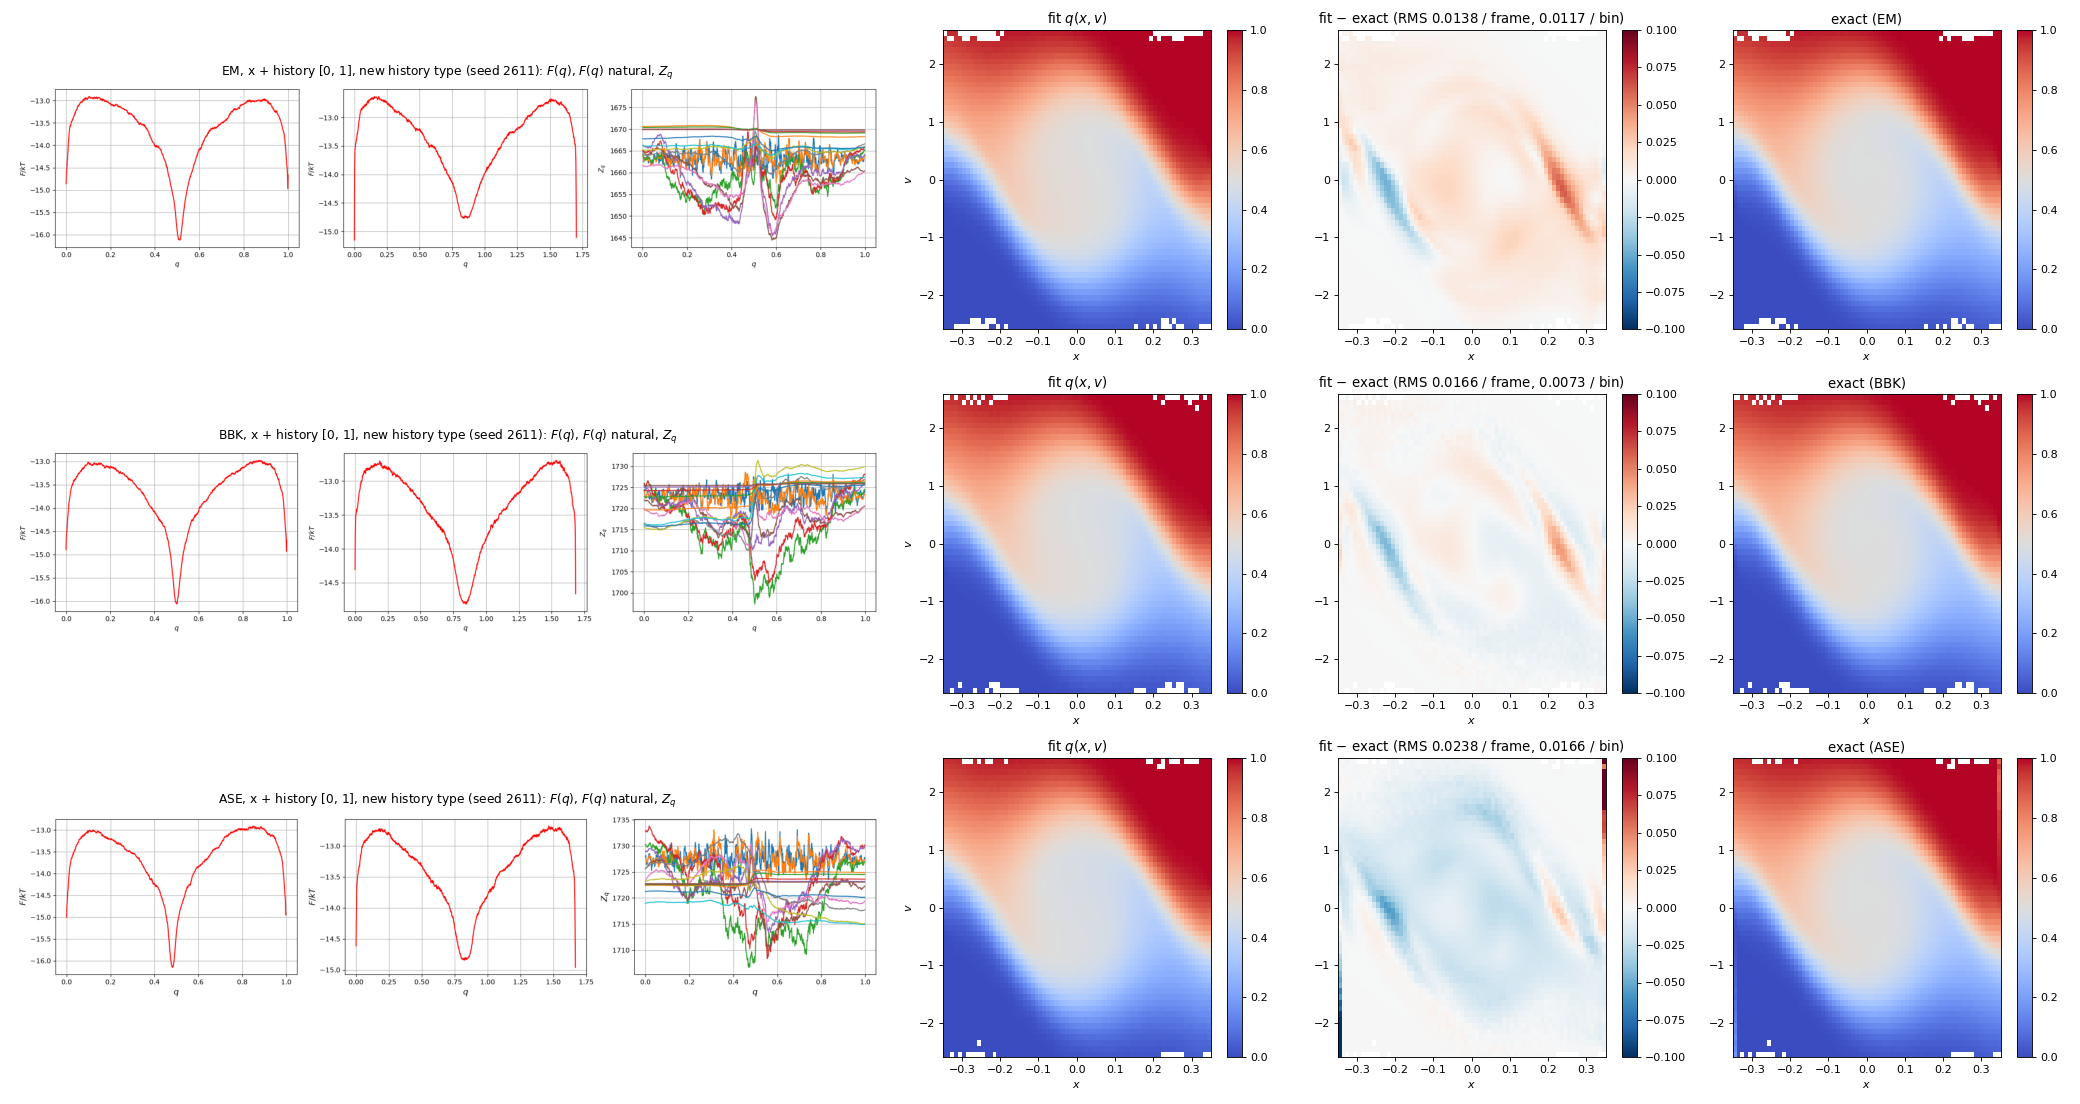
\includegraphics[width=\textwidth]{simple_ry.png}\caption{$x$ + history [0, 1], new history type, seed 2611: $F(q)$, $F(q)$ natural, $Z_q$ \;|\; $q(x,v)$ \;|\; fit $-$ exact \;|\; exact.}
\end{figure}

\section*{Independent EM check}
\texttt{qq\_-Copy1.ipynb}: $dt=0.01$, 3M steps, x + history [0, 1], $\gamma_\mathrm{fit}=0$.
\begin{itemize}
\item $Z_q$ stays within 5100--5165 at every lag, a 1\,\% spread (BBK and ASE history: 20\,\%).
\item Obs-vs-pred lies on the diagonal.
\end{itemize}
\begin{figure}[H]\centering
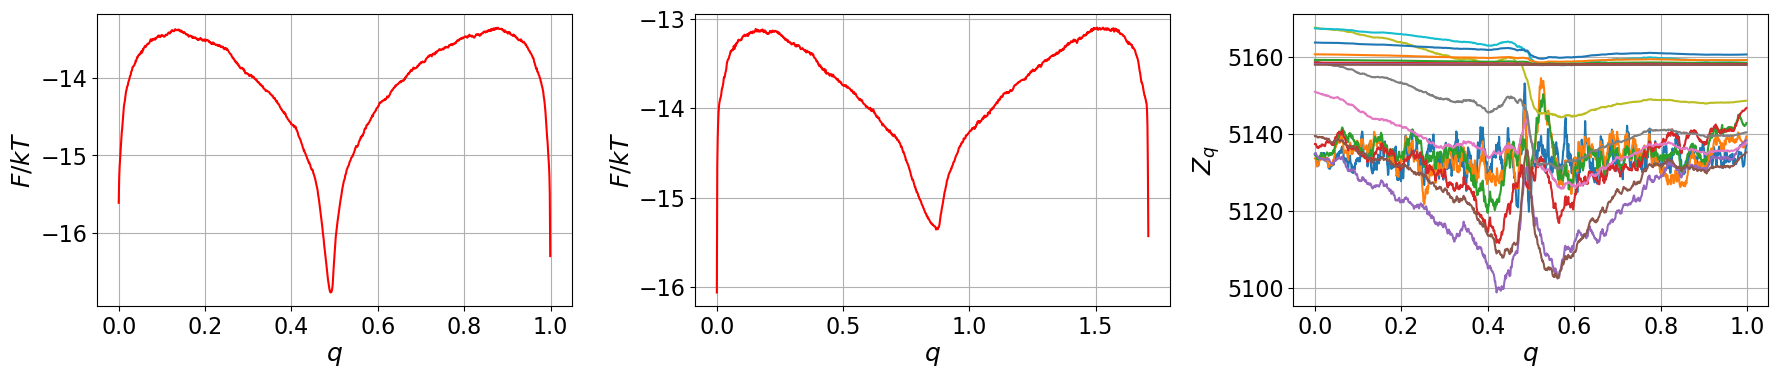
\includegraphics[width=0.66\textwidth]{qq_em_dt0.01/cell1_1.png}\hfill
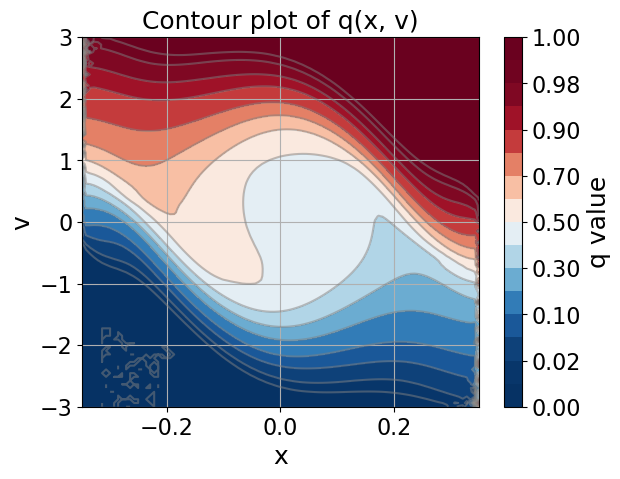
\includegraphics[width=0.32\textwidth]{qq_em_dt0.01/cell1_4.png}
\caption{EM, $dt=0.01$: $F(q)$ and $Z_q$ (left), $q(x,v)$ from x + history [0, 1] (right).}
\end{figure}

\section*{Why the integrator matters}
Notation: $\gamma$ is the friction, $\xi(t)$ the random kick of step $t$, $dt$ the time step, with $\gamma\,dt\ll1$ (here 0.005). $v(t-\tfrac12)$ and $v(t+\tfrac12)$ are the half-step velocities, $\eta(t)$ is a random kick that moves only $x$ (coefficient $c_5$). Forces are left out.

\textbf{EM:} the stored velocity is the one that moved $x$, so positions give it exactly, and $(x(t-1), x(t))$ is Markov.
\[ v(t) = (1-\gamma\,dt)\,v(t-1) + \xi(t), \qquad x(t) = x(t-1) + v(t)\,dt \]

\textbf{BBK and ASE (kick, drift, kick):} the stored velocity gets a second kick after $x$ has moved.
\begin{align*}
v(t-\tfrac12) &= (1-\tfrac{\gamma\,dt}{2})\,v(t-1) + \xi(t)\\
x(t) &= x(t-1) + dt\,v(t-\tfrac12) + c_5\,\eta(t)\\
v(t) &= (1-\tfrac{\gamma\,dt}{2})\,v(t-\tfrac12) + \xi(t)\\
v(t+\tfrac12) &= (1-\tfrac{\gamma\,dt}{2})^2\,v(t-\tfrac12) + (1-\tfrac{\gamma\,dt}{2})\,\xi(t) + \xi(t+1)
\end{align*}
Positions give only $x(t)-x(t-1) = dt\,v(t-\tfrac12) + c_5\,\eta(t)$: the half-step velocity plus a position-only kick, so
even $v(t-\tfrac12)$ cannot be read off them. The stored velocity $v(t)$, the state, gets the same $\xi(t)$ again (ASE) or a
correlated one (BBK, which has the same structure with correlated position and velocity kicks); the last line is the next
half-step velocity.
\begin{itemize}
\item \textbf{Hidden noise:} the position step is one number, $dt\,v(t-\tfrac12)+c_5\eta(t)$. It appears again in $v(t)$ and $v(t+\tfrac12)$.
\item \textbf{Memory:} the residual $\xi(t+1)+(1-\tfrac{\gamma\,dt}{2})\,\xi(t)$ has autocorrelation $\approx\tfrac12$ (for $\gamma\,dt\ll1$). Measured: 0.50 for
  ASE's half-step velocity, 0.25 for the finite-difference velocity of BBK and ASE, 0.00 for EM.
% \item \textbf{Size} (free particle, ASE $\gamma$ and $dt$; share of the velocity noise added per step that $K$ past frames do not
%   determine): exact half-step velocities 0.25, 0.13, 0.03 for $K=1,2,8$ (about $0.25/K$); velocities from position differences
%   0.33, 0.29, 0.29 for $K=1,2,8$, and still 0.29 at $K=128$. The plateau is $c_5\eta$: this is why [0, 1, 2, 4] helps only partly.
  
% \item \textbf{Small in thermal terms, large per step:} about 6\,\% of the thermal speed, but the lag-1 equation works on
%   the per-step scale.
% \item \textbf{Remedy:} fit at a larger lag. BBK with history [0, 1] at fit lag/stride 20 reaches RMS 0.010 per bin
%   (lag 1: 0.031), and $Z_q$ is flat at lags $\ge20$.
\end{itemize}
\end{document}
